\documentclass{sigchi}

% Use this command to override the default ACM copyright statement
% (e.g. for preprints).  Consult the conference website for the
% camera-ready copyright statement.


%% EXAMPLE BEGIN -- HOW TO OVERRIDE THE DEFAULT COPYRIGHT STRIP -- (July 22, 2013 - Paul Baumann)
% \toappear{Permission to make digital or hard copies of all or part of this work for personal or classroom use is      granted without fee provided that copies are not made or distributed for profit or commercial advantage and that copies bear this notice and the full citation on the first page. Copyrights for components of this work owned by others than ACM must be honored. Abstracting with credit is permitted. To copy otherwise, or republish, to post on servers or to redistribute to lists, requires prior specific permission and/or a fee. Request permissions from permissions@acm.org. \\
% {\emph{CHI'14}}, April 26--May 1, 2014, Toronto, Canada. \\
% Copyright \copyright~2014 ACM ISBN/14/04...\$15.00. \\
% DOI string from ACM form confirmation}
%% EXAMPLE END -- HOW TO OVERRIDE THE DEFAULT COPYRIGHT STRIP -- (July 22, 2013 - Paul Baumann)


% Arabic page numbers for submission.  Remove this line to eliminate
% page numbers for the camera ready copy 

%\pagenumbering{arabic}

% Load basic packages
\usepackage{balance}  % to better equalize the last page
\usepackage{graphics} % for EPS, load graphicx instead 
%\usepackage[T1]{fontenc}
\usepackage{txfonts}
\usepackage{times}    % comment if you want LaTeX's default font
\usepackage[pdftex]{hyperref}
% \usepackage{url}      % llt: nicely formatted URLs
\usepackage{color}
\usepackage{textcomp}
\usepackage{booktabs}
\usepackage{ccicons}
\usepackage{todonotes}

% llt: Define a global style for URLs, rather that the default one
\makeatletter
\def\url@leostyle{%
  \@ifundefined{selectfont}{\def\UrlFont{\sf}}{\def\UrlFont{\small\bf\ttfamily}}}
\makeatother
\urlstyle{leo}

% To make various LaTeX processors do the right thing with page size.
\def\pprw{8.5in}
\def\pprh{11in}
\special{papersize=\pprw,\pprh}
\setlength{\paperwidth}{\pprw}
\setlength{\paperheight}{\pprh}
\setlength{\pdfpagewidth}{\pprw}
\setlength{\pdfpageheight}{\pprh}

% Make sure hyperref comes last of your loaded packages, to give it a
% fighting chance of not being over-written, since its job is to
% redefine many LaTeX commands.
\definecolor{linkColor}{RGB}{6,125,233}
\hypersetup{%
  pdftitle={SIGCHI Conference Proceedings Format},
  pdfauthor={LaTeX},
  pdfkeywords={SIGCHI, proceedings, archival format},
  bookmarksnumbered,
  pdfstartview={FitH},
  colorlinks,
  citecolor=black,
  filecolor=black,
  linkcolor=black,
  urlcolor=linkColor,
  breaklinks=true,
}

% create a shortcut to typeset table headings
% \newcommand\tabhead[1]{\small\textbf{#1}}

% End of preamble. Here it comes the document.
\begin{document}

\title{Brainspeedr: A Fast Online Brain-Computer Interface for Rapid Serial Visual Presentation}

\numberofauthors{3}
\author{%
  \alignauthor{1st Author Name\\
    \affaddr{Affiliation}\\
    \affaddr{City, Country}\\
    \email{e-mail address}}\\
  \alignauthor{2nd Author Name\\
    \affaddr{Affiliation}\\
    \affaddr{City, Country}\\
    \email{e-mail address}}\\
  \alignauthor{3rd Author Name\\
    \affaddr{Affiliation}\\
    \affaddr{City, Country}\\
    \email{e-mail address}}\\
}

\maketitle

\begin{abstract}
At the age of online information abundance, the human capacity to retain knowledge is largely limited by the time and the attention required to read text, watch videos, listen to podcasts. For written information, rapid serial visual presentation (RSVP) helps greatly save time with similar levels of text understanding, compared with traditional reading. However, RSVP does not account for attention. We present a simple hybrid brain-computer interface (BCI) that controls in real-time the speed of reading by measuring the instant level of higher cognitive brain activity. Electroencephalogram (EEG) signal is acquired with a single channel consumer-grade headset and analyzed in the frequency domain. The pace of word display is controlled by a measure brainwave entropy. We have conducted a controlled experiment with 50 subjects with three distinct treatments, and we show that brain-controlled speed-reading increases the speed and the understanding of texts by subjects.
\end{abstract}

\keywords{brain-computer interface (BCI); electroencephalogram (EEG); human cognition; usability testing}


\category{H.1.2}{User/Machine Systems}{Miscellaneous} \category{J.3}{Life and Medical Sciences}{}{}s
%\category{H.5.m.}{Information Interfaces and Presentation
%  (e.g. HCI)}{Miscellaneous} \category{See
%  \url{http://acm.org/about/class/1998/} for the full list of ACM
%  classifiers. This section is required.}{}{}

\section{Introduction}
\section{Related Work}

\subsection{RSVP}



\subsection{Brainwaves}




\section{Apparatus}
The brain speed-reader is an apparatus, which displays words on a screen at variable $r(t)$, which in turn is read by the user. The reading task triggers a change of brain activity, which can be recorded and analyzed through electroencephalograms (EEG). As our apparatus is conceived for use in a naturalistic environment, we have used, {\it Neurosky Mindwave}, the cheapest consumer-grade EEG headset available for less than \$100 on the market. As shown on Figure \ref{fig:apparatus} and explained step-by-step below, the EEG signal is processed online, in order to adapt the rate of words displayed as function of cognitive activity: if the rate $r$ is too large (resp. too low) at time $t$, then reading triggers more  (resp. less) cognitive activity, which in turn allows reducing (resp. increasing) $r$ at $t+1$. In this section, we explain step-by-step the design of the apparatus in details.

\begin{figure}[!t]
\centering
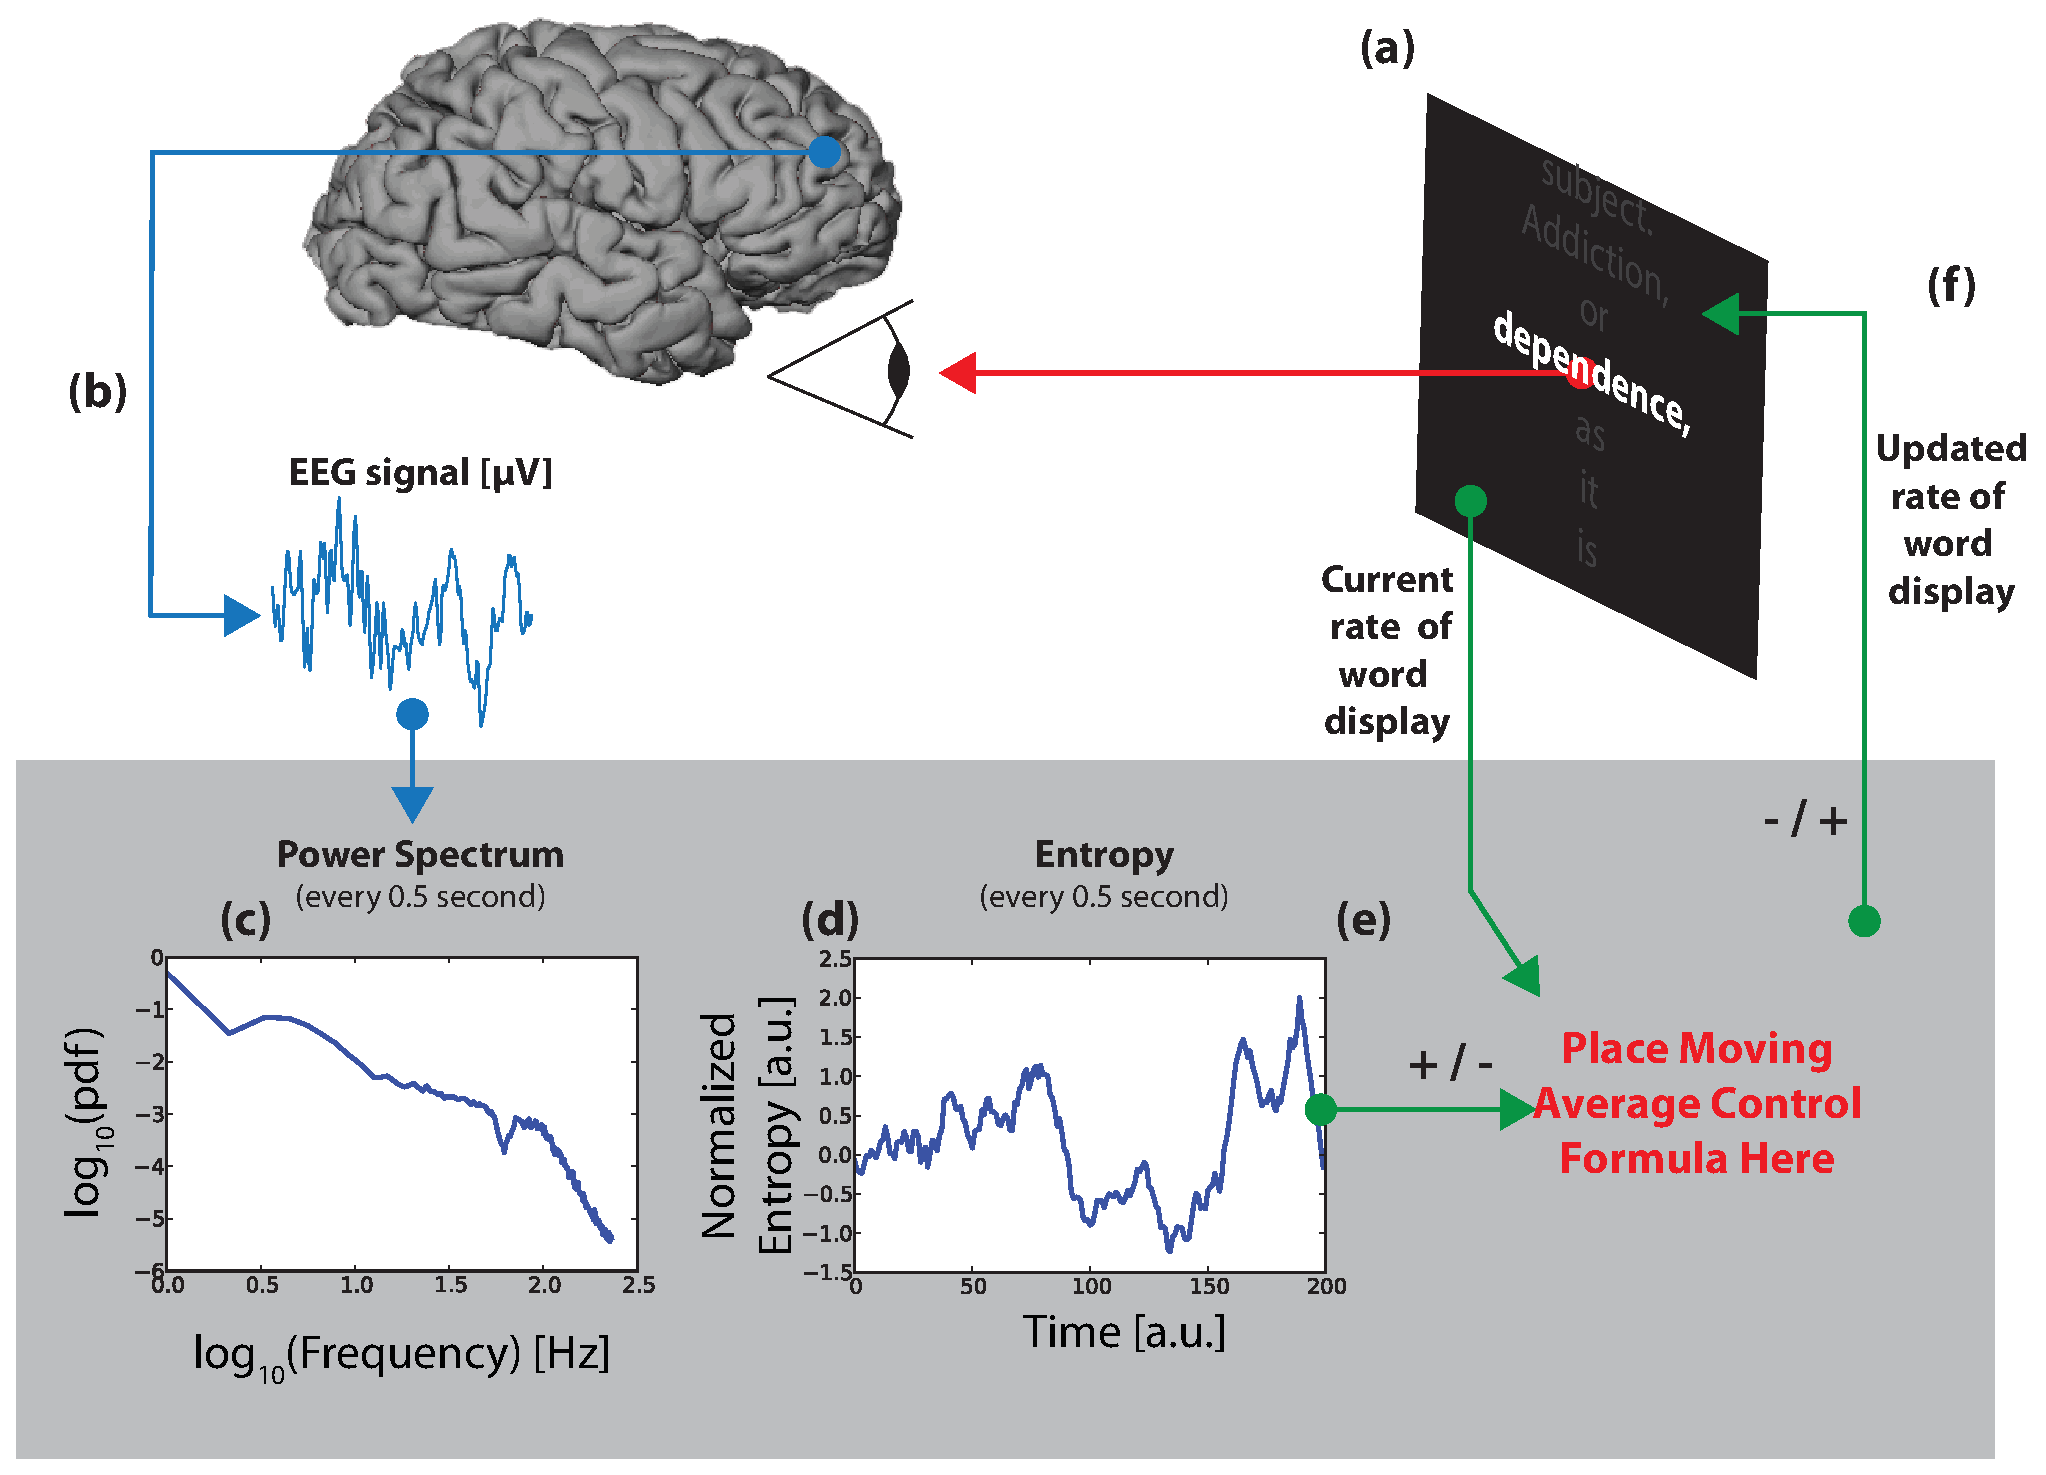
\includegraphics[width=0.9\columnwidth]{../figures/apparatus.eps}
\caption{Brain speed-reader apparatus: {\bf (a)} Words are displayed and read one after the other at a given rate. {\bf (b)} the EEG signal is recorded through a consumer grade device (here the {\it Neurosky Mindwave}). {\bf (c)} The EEG signal is turned every 0.5 seconds into a power spectrum through a Fourier transform, {\bf (d)} the characteristics of the power spectrum are compressed into a single value characteristic entropy $s$ value. {\bf (e)} A new rate of word display is updated by taking into its current value and $s$. {\bf (f)} The rate of word display is updated accordingly.}
\label{fig:apparatus}
\end{figure}

\subsection{Rate of Word Display}
The principle of {\it Rapid Serial Visual Presentation} (RVSP) applied to text, is precisely to display the words of a text at a controlled rate. However, in most RVSP implementations for text, the rate of word display pre-determined and remains constant. In our implementation, the user first calibrates the brain speed-reader by tuning a comfortable baseline word display rate $r_{baseline} = r(t = 0)$. The operation takes only a few seconds. This is a usual way to proceed when using usual text RVSP applications.

\subsection{Brain Activity as Captured by EEG signal}
Unlike traditional text RVSP, we wish to let the user adapt the rate of word display in real-time, through brain activity as captured by EEG signal, to control for a text becoming suddenly becoming more difficult, or just because the mindset of the user has changed, like sudden focus on an important part of the text (lower rate desired) or, on the contrary, loss of attention (higher rate of word displayed desired).

Because we want our apparatus be usable outside the lab, we have chosen the cheapest consumer-grade EEG scanner, available on the market for less than \$100.

\subsection{EEG Signal Processing}
One way to process the EEG signal, consists in analyzing its spectral properties over a determined period. Here, we take a time window of 0.25 second, which allows us to analyze the frequency domain $0-128Hz$, since the sampling rate of the Neurosky Mindwave is 512 measures per second (i.e., 512 Hz). Hence, every 0.25 second, we compute the power spectrum given by, 

 \begin{equation}
\label{eq:pspectrum}
\mathbf{[pspectrum~here]}
\end{equation}
 
and which is expected to approximately follow a power law, i.e., the probability to find a frequency $x$ is given by the probability density function $pdf(x)  = 1/x^{\mu+1}$. The power spectrum varies as a function of the mental tasks occurring, and potential external perturbations, such as voice, imperceptible and perceptible muscle movements, eye-movement, blinking.


\begin{figure}[!t]
\centering
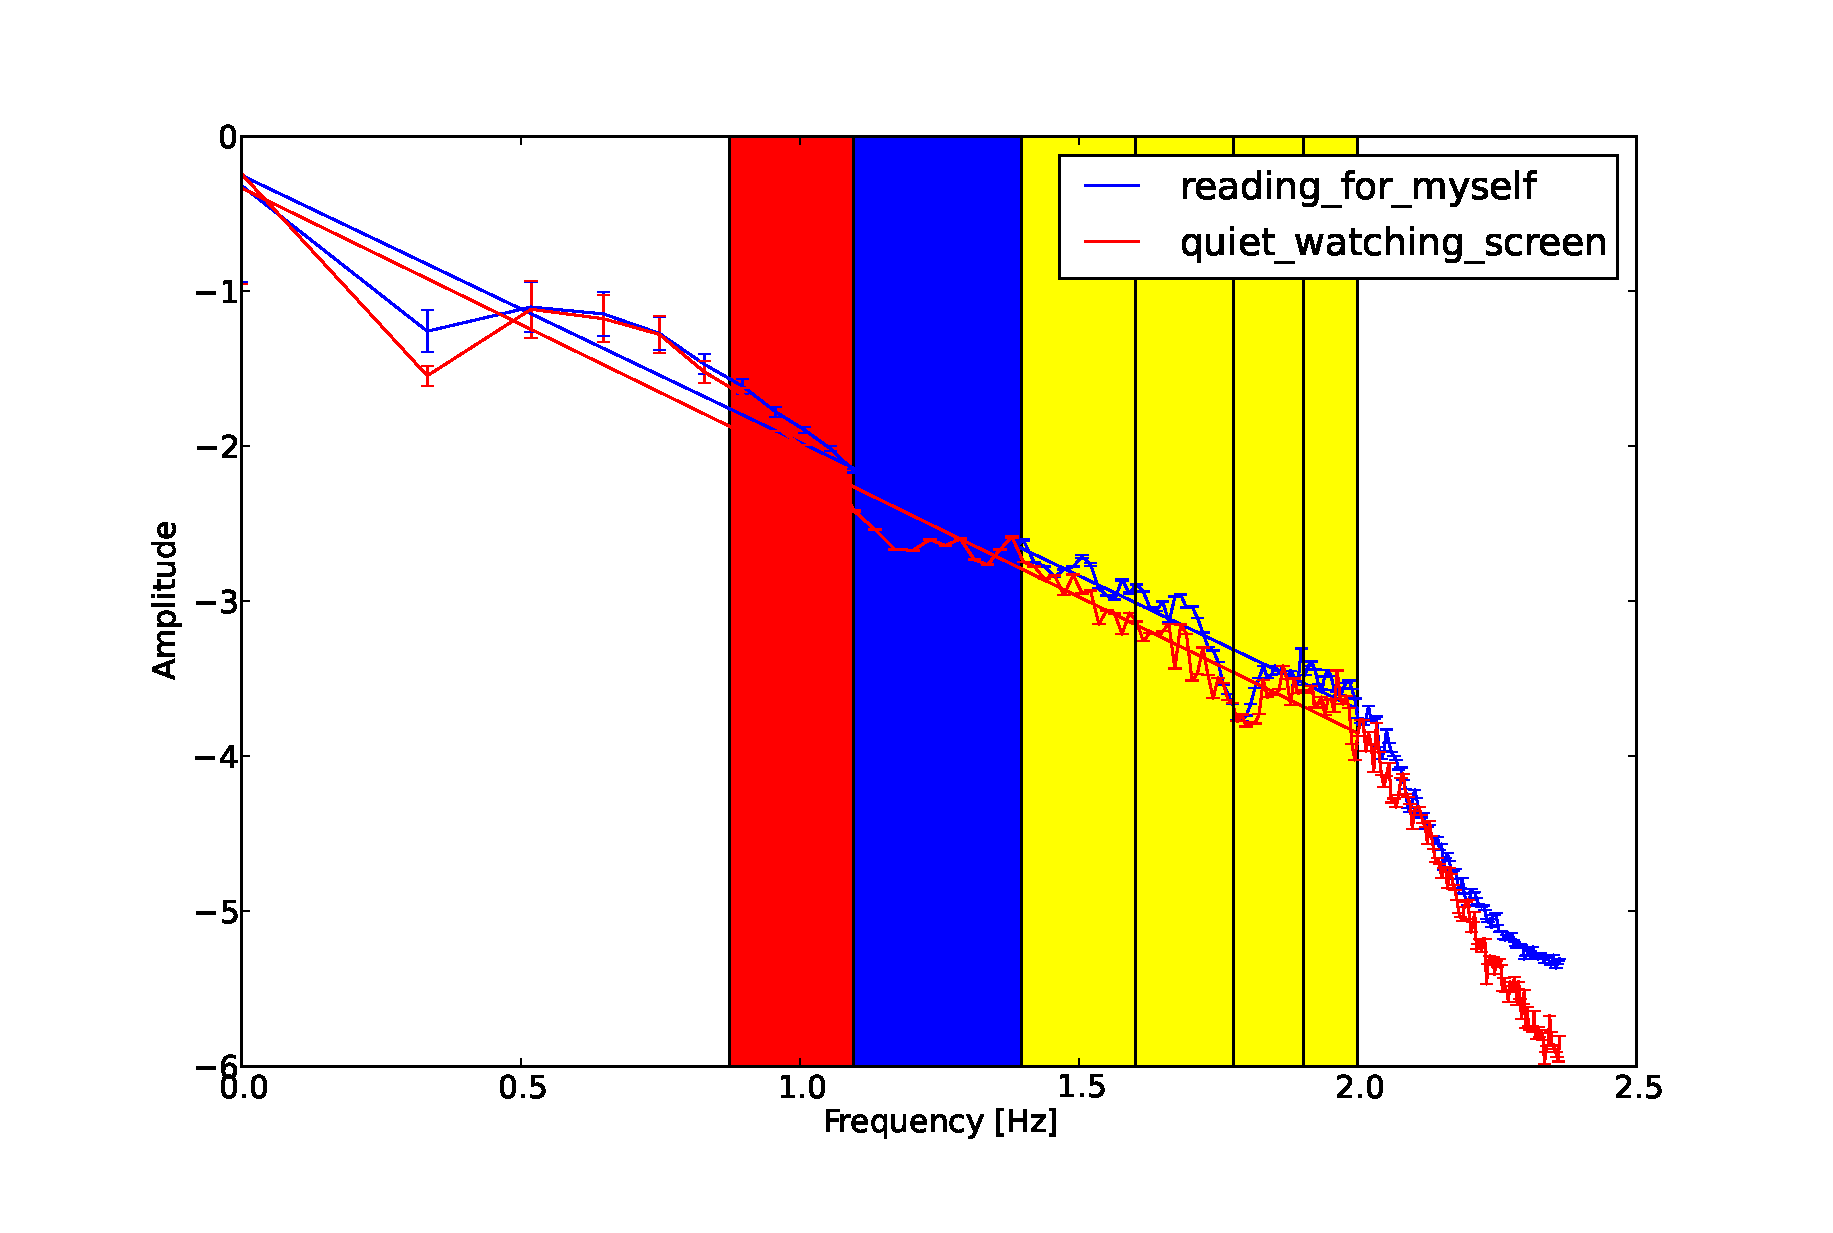
\includegraphics[width=0.9\columnwidth]{../figures/compare_pSpectra.eps}
\caption{Comparison of power spectra of a subject (i) resting state and (ii) reading a text in English for himself. {\bf [report the entropy values in both cases]}}
\label{fig:pspectrum}
\end{figure}


Then, entropy.

\begin{equation}
\label{eq:tsallis}
S_q(X) = \frac{1}{q-1} \left( 1 - \sum_{i=1}^n (p_i)^q \right).
\end{equation}

\begin{equation}
\label{eq:shannon}
S_1(X) = - \sum_{i=1}^n p_i\cdot log_{2}(p_i), ~~for~~q=1.
\end{equation}

\subsubsection{Why Entropy ?}

higher frequencies are usually associated to higher cognitive brain activation. Higher activation  translated into larger entropy $S$.


We wanted a lightweight mobile apparatus, which does not require complicated machine learning or any communication with a cloud service, or would not drain a battery. We purposely decided for a cheap update method {\bf [continue this point in discussion because it helps introduce future work]}

\begin{figure}[!t]
\centering
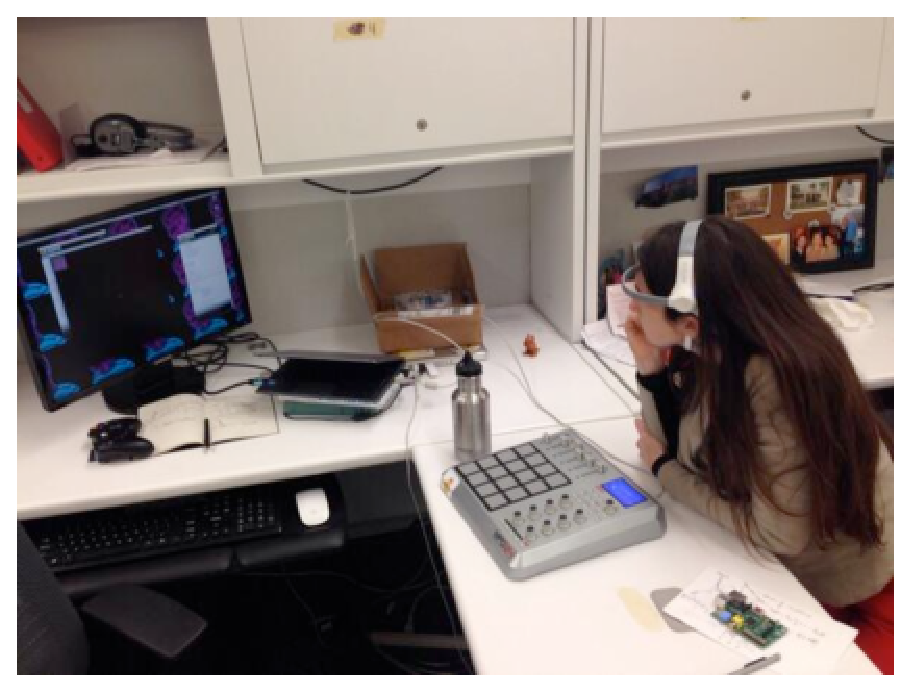
\includegraphics[width=0.9\columnwidth]{../figures/ariel.eps}
\caption{Ariel Garten (Interaxon / Muse CEO) playing with the brain speed reader.}
\label{fig:ariel}
\end{figure}

One could argue that we could have taken the {\it meditation} and {\it attention} metrics provided by Neurosky (and computed directly in the headset). However, these metrics are proprietary and their formula kept secret (we suspect nevertheless that they take $\alpha$ and $\beta$ waves  as an input). Furthermore, extensive testing did not allow us find any consistency with what we would quality meditation or attention. As a result, we preferred to stick to the principles of reproducible science.

\subsection{Negative Feedback Loop}

Explain: higher cog. activity  $\rightarrow$  higher entropy $\rightarrow$  lower word display rate $\rightarrow$ lower cog. activity. {\bf [probably not worth a section]}


\subsection{Word Display Rate Update}

\begin{equation}
\label{eq:Snormalized}
S_{norm}(t) = \frac{S(t) - \langle S \rangle}{\sigma_{S}}, 
\end{equation}
with $\langle S \rangle$ and $\sigma_{S}$ the average and standard deviation of the entropy $S$ calculated over the last 20 points (i.e., the last 5 seconds?). The normalization ensures that $S_{norm}$ is always centered around $0$. The rate $R(t+1)$ of word display is then updated as follows,

\begin{equation}
R(t+\Delta t) = R(t) \left[1 - \alpha \cdot S_{norm}(t)\right],
\label{eq:RateChange}
\end{equation}

where $\Delta t = 0.25$ seconds and $\alpha = 0.20$. In other words, the normalized entropy influences for 20\% the rate change $\Delta R =  \left[ R(t+\Delta t) - R(t) \right] / R(t) = - \alpha \cdot S_{norm}(t)$. Increasing $\alpha$ increases the influence of $S_{norm}$, and the negative sign ensures control of $R$ with a mean reverting process. Note however, that since $S_{norm}$ is calculated from a moving average on a rather short time window, $R$ exhibits excursions (c.f. Figure \ref{fig:trajectory}).

\begin{figure}[!t]
\centering
%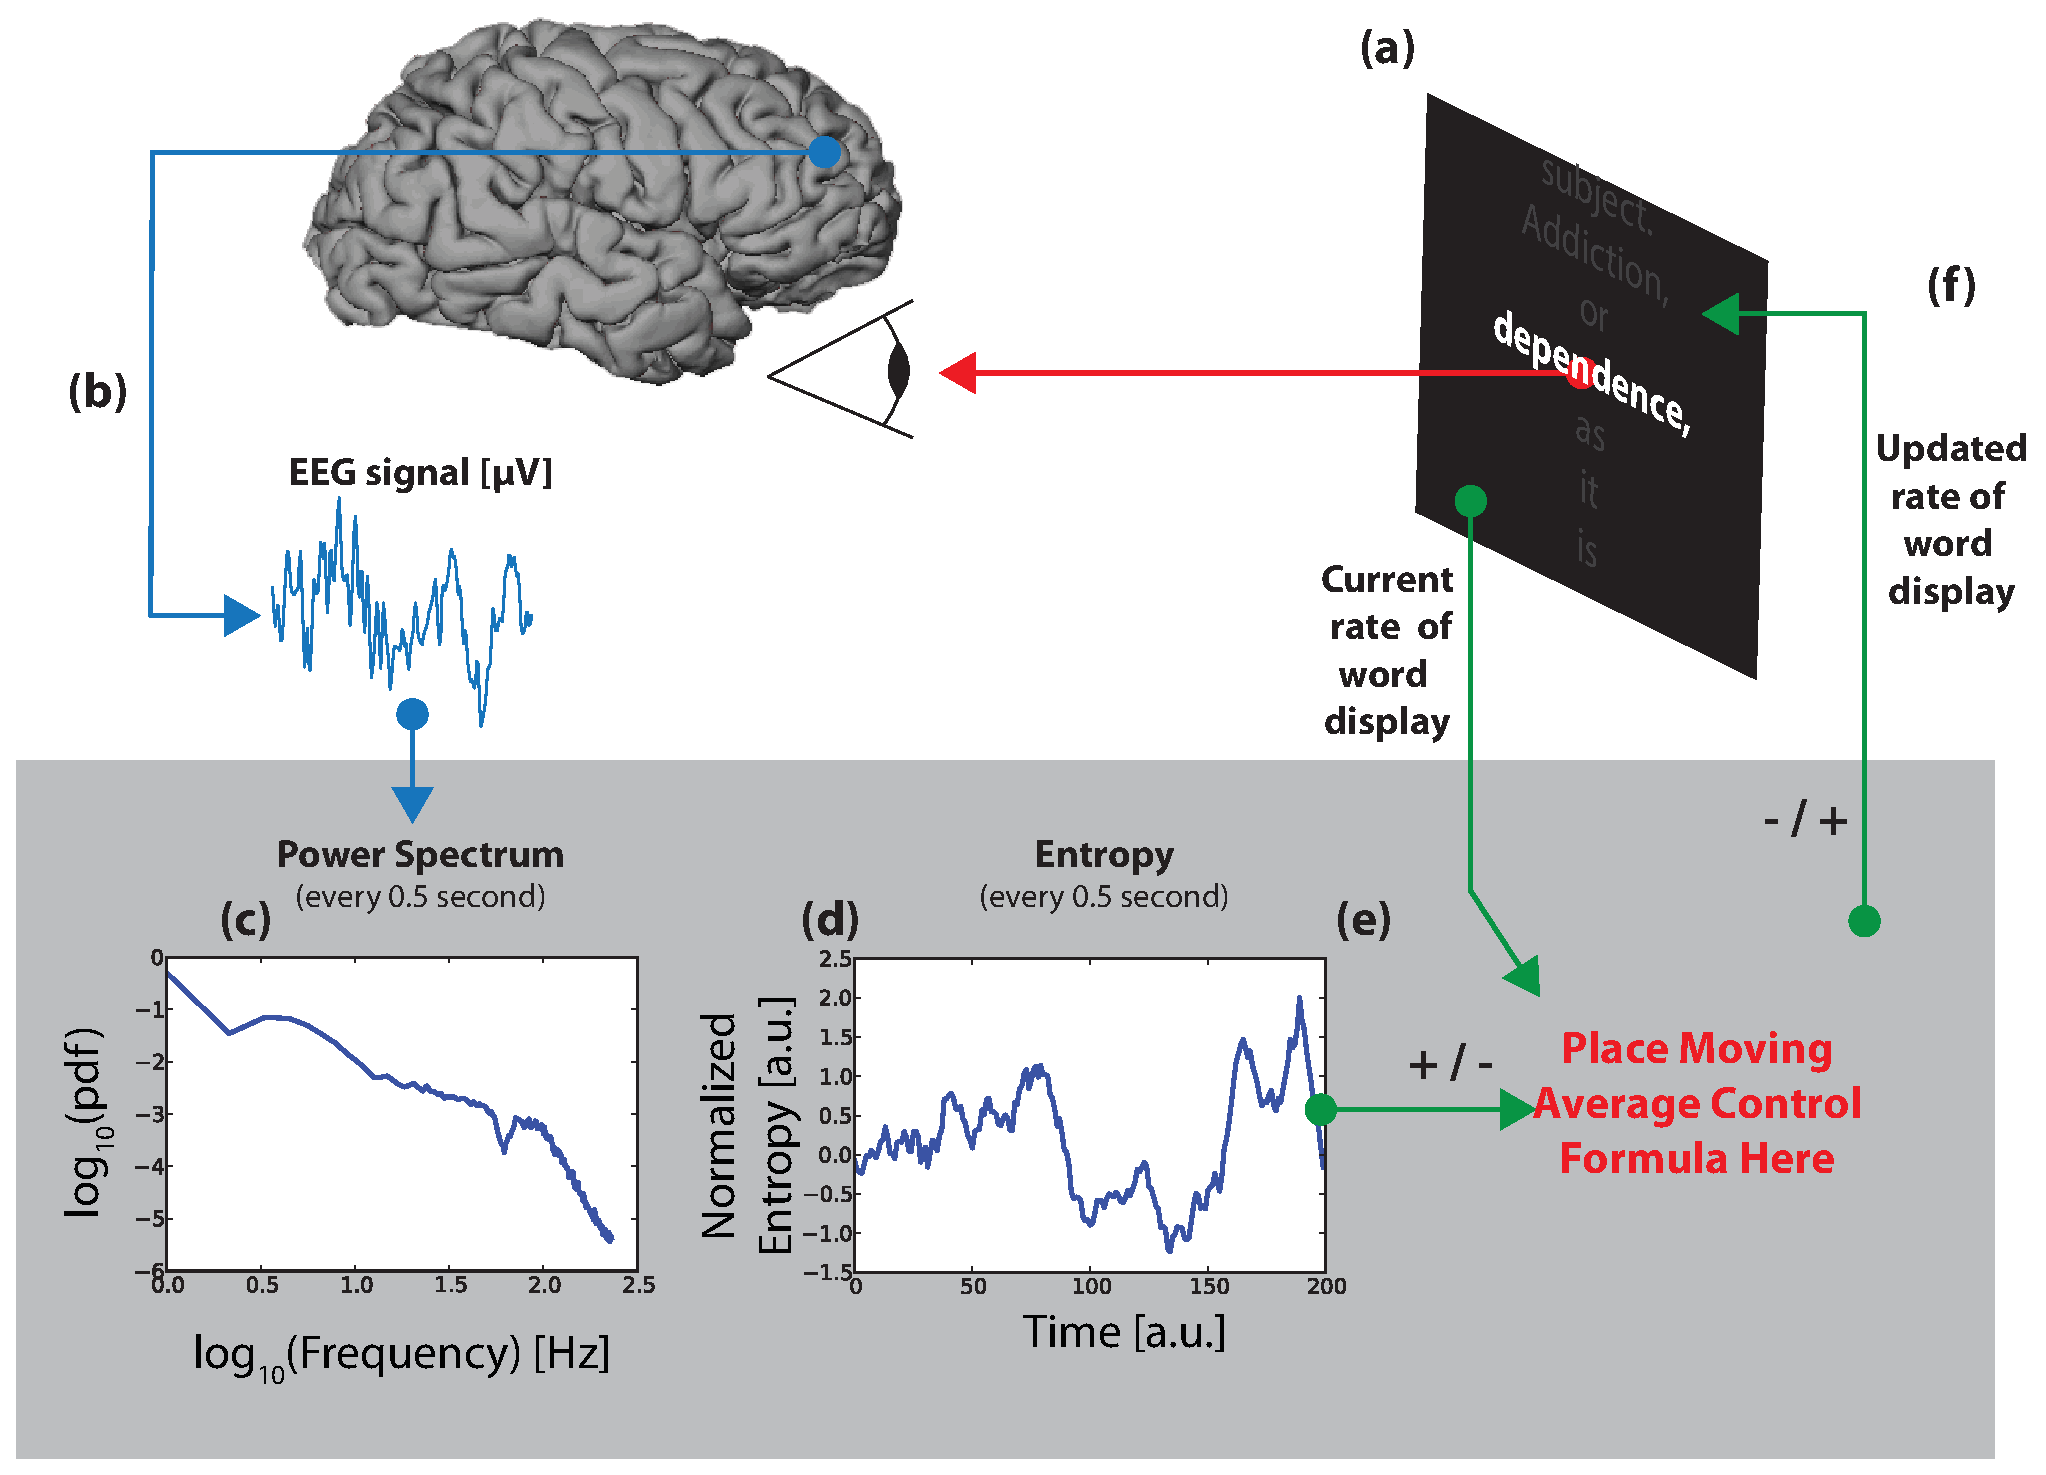
\includegraphics[width=0.9\columnwidth]{../figures/apparatus.eps}
\caption{typical evolution of rate $R$.}
\label{fig:trajectory}
\end{figure}

\section{Method}

\subsection{Brain Speed Reader}

{\bf describe the brain control system}

\begin{enumerate}
  \item capture brainwaves for 1 second
  \item compute power spectrum
  \item compute normalized entropy
  \item update display speed ({\bf trick of the moving average to be described here})
\end{enumerate}


\subsection{Experimental Protocol}


\begin{enumerate}
  \item Constant Rate
  %\item Randomly Varying Text : AR(1) $\rigtharrow$ AR1(n,baseline,baseline/2,0.5,sigma=std) AR1 formula : $c + phi * X[-1] + np.random.normal(scale=sigma)$
  %\item Brain Speed Reader : (i) compute entropy $S$ at t, (ii) normalize $S$ as $S_{norm} = (S- \langle S \rangle) / \sigma_S$, with $\langle S \rangle$ and $\sigma_S$ computed over the last XX values of entropy, (iii) compute a new speed as $v(t+1) = v(t)\cdot(1-0.2\sdot S_{norm})$
\end{enumerate}


\subsection{Measuring Text Complexity}

ATOS  ( ref: Michael Milone,The Development of ATOS, The Renaissance Readability Formula, p10 (2010) \url{http://doc.renlearn.com/KMNet/R004250827GJ11C4.pdf}

\begin{itemize}
  \item Words per sentence
  \item Average grade level of words ( which class grade the word is first seen)
  \item Characters per word
\end{itemize}


$ATOS Rasch Difficulty Formula = -8.54 + 1.95 * Ln(AvgWords) + .46 * AvgGrad100 + 1.74 * Ln(AvgChar)$

Adjustment for books with less than 500 words

$BLGL for Books With Fewer Than 500 Words = .004 * Book Length + 0.4$


Table detailing texts : \url{https://docs.google.com/spreadsheets/d/1uwkoToM-p3UFrd0U_1vOX4eBJsmYuPVYVhvhsZ8Y5Nc/edit#gid=0}




%\begin{itemize}
%  \item {\bf text 0 (adapted from Coming of Age in Samoa, Margaret Mead, 1928
%)}:   $ATOS=9.5$,  $word~count = 421$
%  \item {\bf Text 1  (adapted from The Warden, Anthony Trollope, 1855)} : $ATOS=8.3$, $word~count = 563$
%  \item {\bf Text 2  (adapted from The Mayor of Casterbridge, Thomas Hardy, 1886) } : $ATOS=10.2$, $word~count = 831$
%  \item {\bf Text 3 (Adapted from: The Social Function of Science, John D Bernal (1939))} : $ATOS=11.9$, $word~count = 421$
%\end{itemize}


\input{sections/data}
\section{Results}
\label{results}


For $17$ over $21$ participants, the RSVP rate was characterized by a balanced joint probability of {\it rate change x word size frequency} in treatment (ii) and (iii) (Fig. 2a). Long words triggered the largest change of entropy (resp. rate), while words smaller than the average size ( $< 5.5$ characters) were associated with reverse entropy (resp. rate) change (Fig. 2b, 2c).\\

Despite the large variation of entropy, texts could be decoded by matching the sequence of entropy measures (associated with each word) with the unique sequence of word lengths (Fig 3). Our results did not require preliminary identification of participants, and the success rate was 27.4\%, roughly 11\% above chance (i.e., $1/6 \approx 16.67\%$), when considering the first 300 words of each text.



\begin{itemize}
  \item performance*, perceived comfort and control as a function of treatment 
  \item for brain speed reader treatment:  performance*, perceived comfort and control as a function $X_0$, $alpha$
\end{itemize}

*performance means either {\bf conceptual} (understanding the meaning), {\bf conceptual-memory} (recalling characters) or {\bf memory} (recalling some words).


\section{Discussion}
\label{discussion}
Recognizing the importance of reading more in less time, while avoiding multi-tasking, we have put to the test the {\it brain speed reader}, a brain-computer interface (BCI) implementing a rate varying rapid serial visual presentation (RSVP) of text words. We have found that a majority of users who participated in our study could control the brain speed reader. Furthermore, we found that roughly half of participants could self-regulate with two opposite control mechanisms ({\it bsr+} and {\it bsr-}). The achievement of self-regulation is negatively influenced by age, text length, topic familiarity and speed reading comfort. Self-regulation achievement (stability) is however highly positively correlated with reading pleasure. Capacity to provide a meaningful text summary {\it ex-post} (the best way to test for text comprehension) is also positively associated with stability, yet in a weakly significant way.

Our results show that the brain speed reader is an adequate technology to foster fast knowledge integration in a world of abundant information and endless news feeds, while at the same time helping preventing multi-tasking. The design implements self-regulation neurofeedback as a way to ensure that users concentrate on reading the text: If the user does not or cannot concentrate, the RSVP rate will drift towards very slow (resp. fast) word display rates. Multi-tasking is discouraged by design, and reading speed is doubled compared to normal reading.

Self-regulation neurofeedback stems from the capacity by the brain to train and adapt its wave modulations in order to perform specific tasks better \cite{piano_neurofeedback}, or to reach desired mental states \cite{neurofeedback_meditation}.  As a special kind of neurofeedback BCI, the brain speed reader may be help remediate reading disabilities or difficulties associated with a lack of concentration capabilities, which is one consequence of multi-tasking. Because the brain speed reader (BSR) does not require prior calibration, training and use occur concomitantly: Either the user achieves self-regulation quickly and then {\it uses} BSR, or she remains in training mode until she reaches self-regulation. In our experiment, we have set very large boundary for slowest (resp. fastest) RSVP rate to make sure that subjects who reach the boundaries effectively failed achieving self-regulation. In training mode, these RSVP rate boundaries may be tuned and personalized to ensure that the user can reach a compromise between attempts to achieve self-regulation and still reading fast with pleasure while training. While we have not tested medical applications for the brain speed reader, it may help users suffering from dyslexia or attention disorder and hyperactivity disorders (ADHD) improve their reading and their attention.

\subsection{Limitations}
The version of the brain speed reader presented here is a first attempt to harness self-regulated neurofeedback for the sake of upgrading the reading experience to arising challenges in society, such as tackling the abundance of natural language- written information while reducing multi-tasking. Although our first experiment show encouraging results, we have come up with the simplest possible implementation and experimental protocol. A number of outstanding questions remain and deserve further work, starting with the hardware we used. Neurofeedback most often involves a limited number of EEG electrodes, but typically of higher quality and on other positions in the 10-20 system. One may want to experiment with a variety of electrode quality, number, and positions to elicit a better hardware configuration.

Our study bears a number of limitations regarding comprehension and memory. We did not find a significant difference of comprehension between RSVP speed read at constant rate versus {\it bsr+} and {\it bsr-} treatments. We find a slight comprehension improvement when users achieve more stable self-regulation, but this result need further validation, presumably with a larger data set. We have also not measured how comprehension and word recall are diminished (resp. increased) as reading speed doubles, i.e., when comparing brain speed reading and reading text normally. Previous research suggests that comprehension is diminished by constant RSVP rate speed reading \cite{kujala2007phase}, although it remains the same or is slightly improved for people with reading disabilities. Further investigation is required to better elicit how self-regulation stability influences comprehension and word recall

We shall also investigate why some participants could not achieve self-regulation: It remains unclear if they had indeed to train further before making it right, or if the BSR parameters we chose [initial RSVP rate $X(t=0) = 125$ ms/word and $|\alpha| = 0.005$] may only be suitable for a subset of the population, and may require further adaptation. Similarly, we have no information on the time it takes to learn given that the user could not achieve self-regulation at once. We chose $X(t=0) = 125$ ms/word as the starting RSVP rate, which is also the value known to be most comfortable on average to people who read with RSVP. To further understand and validate the self-regulation mechanism, it would be desirable to perform additional investigations with a variety of starting rates. Our hypothesis is that within a yet unknown RSVP rate range, users capable of self-regulation can stabilize the rate, while beyond some limits it is impossible to control the brain speed reader, in particular when the presentation speed is high. It also remains to be seen if users tend to stabilize the rate close to 125ms/word on average, even if the initial RSVP rate is smaller (resp. larger).

Even though there is no need for preliminary {\it ad-hoc} calibration to use the brain speed reader, learning still occurs ``on the fly", with several advantages as already mentioned above. It would nevertheless be desirable to better understand how the user transitions from {\it learning} to {\it using}. This has implications for more elaborate and personalized UX design.

Finally, we found that text length has a negative effect on self-regulation stability (roughly one unit per 1300 words as shown in Table \ref{tab:reg}). This is a concern because the brain speed reader is supposed to let users avoid multi-tasking to concentrate on a single task instead. Here, it appears that if the task lasts too long, then self-regulation undergo changes of regime and reduced stability. This suggests that either BSR is suited for {\it long but not that long tasks} and/or there is another factor involving learning how to keep self-regulation highly stable over long tasks. This is has further implications on comprehension and memory, which need to be further addressed.

\subsection{Beyond speed reading}
Here, we have designed and tested brain-computer interface (BCI), which helps seamlessly control the parsing rate of a coherent sequence of a words as visual stimuli. The same time varying rate RSVP coupled with a neurofeedback BCI may be used beyond reading. It could apply similarly to cartoons, video or audio streams, if the control is made on the continuous speed (i.e., the pitch) of the media stream, similarly to the (discrete) presentation rate used in our experiment.

Similar BCI could be used to assess the quality and the coherence of a piece of text. Indeed, it appears that when reading, the brain makes some heuristic predictions of what word(s) is (resp. are) coming next \cite{smith2013effect}. Unexpected words trigger an unusual cognitive activity which slows the reading. Recording how the effects of unexpected stimuli materialize in conjunction with control remain yet to the be investigated. 

%\section{Future Work}
\section{Conclusion}
\label{conclusion}
%Recognizing the importance of reading more in less time, while avoiding multi-tasking, a way to do more in less time, yet most often at the cost of less grasp on tasks at hand

In this article, we have proposed, designed and tested a new approach to brain computer interfaces, geared towards handling and controlling a fast-paced flow of information in way that limits diversion from the focal taks and hence, prevents multi-tasking. Our approach is based on a peculiar and seldom phenomenon occurring in the brain -- known as {\it self-regulation}. This phenomenon can be assimilated to independent neurofeedback. We have then tested and benchmarked the so-called {\it brain speed reader} in the context of reading text, and we have found that a large proportion of participants to our experiment successfully achieved self-regulation without prior training for at least one of both treatments proposed. On average they would read twice as fast as with normal reading. We furthermore found that age, text length and speed reading comfort have a negative effect on the achievement of self-regulation. On the contrary, capacity to read fast in a normal setting, and reading pleasure have a positive impact on stability. The pleasure in reading suggests the existence of a reward mechanism when a participant achieves self-regulation. Comprehension is only weakly improved when self-regulation is achieved. 

%``It would elevate the computer to a genuine prosthetic extension of the brain" (Vidal 1973)
%``(to identify appropriate correlates of mental states and decisions in external signals" (Vidal 1973)


%\begin{abstract}
%  UPDATED---\today. This sample paper describes the
%  formatting requirements for SIGCHI conference proceedings, and
%  offers recommendations on writing for the worldwide SIGCHI
%  readership. Please review this document even if you have submitted
%  to SIGCHI conferences before, as some format details have changed
%  relative to previous years. Abstracts should be about 150 words and
%  are required.
%\end{abstract}
%

%
%\section{Introduction}
%
%This format is to be used for submissions that are published in the
%conference proceedings. We wish to give this volume a consistent,
%high-quality appearance. We therefore ask that authors follow some
%simple guidelines. You should format your paper exactly like this
%document. The easiest way to do this is to replace the content with
%your own material.  This document describes how to prepare your
%submissions using \LaTeX.
%
%\section{Page Size and Columns}
%On each page your material should fit within a rectangle of 7 $\times$
%9.25 inches (18 $\times$ 23.5 cm), centered on a US Letter page (8.5
%$\times$ 11 inches), beginning 0.75 inches (1.9 cm) from the top of
%the page, with a 0.33 inches (0.85 cm) space between two 3.3 inches
%(8.4 cm) columns. Right margins should be justified, not
%ragged. Please be sure your document and PDF are US letter and not A4.
%
%
%\section{Typeset Text}
%The styles contained in this document have been modified from the
%default styles to reflect ACM formatting conventions. For example,
%content paragraphs like this one are formatted using the Normal style.
%
%
%\LaTeX\ sometimes will create overfull lines that extend into columns.
%To attempt to combat this, the \texttt{.cls} file has a command,
%\texttt{{\textbackslash}sloppy}, that essentially asks \LaTeX\ to
%prefer underfull lines with extra whitespace.  For more details on
%this, and info on how to control it more finely, check out
%{\url{http://www.economics.utoronto.ca/osborne/latex/PMAKEUP.HTM}}.
%
%\subsection{Title and Authors}
%
%Your paper's title, authors and affiliations should run across the
%full width of the page in a single column 17.8 cm (7 in.) wide.  The
%title should be in Helvetica or Arial 18-point bold.  Authors' names
%should be in Times New Roman or Times Roman 12-point bold, and
%affiliations in 12-point regular.  
%
%See \texttt{{\textbackslash}author} section of this template for
%instructions on how to format the authors. For more than three
%authors, you may have to place some address information in a footnote,
%or in a named section at the end of your paper. Leave one 10-point
%line of white space below the last line of affiliations.
%
%\subsection{Abstract and Keywords}
%
%Every submission should begin with an abstract of about 150 words,
%followed by a set of Author Keywords and ACM Classification
%Keywords. The abstract and keywords should be placed in the left
%column of the first page under the left half of the title. The
%abstract should be a concise statement of the problem, approach, and
%conclusions of the work described. It should clearly state the paper's
%contribution to the field of HCI\@.
%
%\subsection{Normal or Body Text}
%
%Please use a 10-point Times New Roman or Times Roman font or, if this
%is unavailable, another proportional font with serifs, as close as
%possible in appearance to Times Roman 10-point. Other than Helvetica
%or Arial headings, please use sans-serif or non-proportional fonts
%only for special purposes, such as source code text.
%
%\subsection{First Page Copyright Notice}
%This template include a sample ACM copyright notice at the bottom of
%page 1, column 1.  Upon acceptance, you will be provided with the
%appropriate copyright statement and unique DOI string for publication.
%Accepted papers will be distributed in the conference
%publications. They will also be placed in the ACM Digital Library,
%where they will remain accessible to thousands of researchers and
%practitioners worldwide. See
%\url{http://acm.org/publications/policies/copyright_policy} for the
%ACM’s copyright and permissions policy.
%
%%%%
%
%\subsection{Subsequent Pages}
%
%On pages beyond the first, start at the top of the page and continue
%in double-column format.  The two columns on the last page should be
%of equal length.
%
%\begin{figure}
%\centering
%  \includegraphics[width=0.9\columnwidth]{figures/sigchi-logo}
%  \caption{Insert a caption below each figure. Do not alter the
%    Caption style.}~\label{fig:figure1}
%\end{figure}
%
%\subsection{References and Citations}
%
%Use a numbered list of references at the end of the article, ordered
%alphabetically by last name of first author, and referenced by numbers
%in
%brackets~\cite{acm_categories,ethics,Klemmer:2002:WSC:503376.503378}.
%Your references should be published materials accessible to the
%public. Internal technical reports may be cited only if they are
%easily accessible (i.e., you provide the address for obtaining the
%report within your citation) and may be obtained by any reader for a
%nominal fee. Proprietary information may not be cited. Private
%communications should be acknowledged in the main text, not referenced
%(e.g., ``[Borriello, personal communication]'').
%
%References should be in ACM citation format:
%\url{http://acm.org/publications/submissions/latex_style}. This
%includes citations to internet
%resources~\cite{acm_categories,cavender:writing,CHINOSAUR:venue,psy:gangnam}
%according to ACM format, although it is often appropriate to include
%URLs directly in the text, as above.
%
%
%% Use a numbered list of references at the end of the article, ordered
%% alphabetically by first author, and referenced by numbers in
%% brackets~\cite{ethics, Klemmer:2002:WSC:503376.503378,
%%   Mather:2000:MUT, Zellweger:2001:FAO:504216.504224}. For papers from
%% conference proceedings, include the title of the paper and an
%% abbreviated name of the conference (e.g., for Interact 2003
%% proceedings, use \textit{Proc. Interact 2003}). Do not include the
%% location of the conference or the exact date; do include the page
%% numbers if available. See the examples of citations at the end of this
%% document. Within this template file, use the \texttt{References} style
%% for the text of your citation.
%
%% Your references should be published materials accessible to the
%% public.  Internal technical reports may be cited only if they are
%% easily accessible (i.e., you provide the address for obtaining the
%% report within your citation) and may be obtained by any reader for a
%% nominal fee.  Proprietary information may not be cited. Private
%% communications should be acknowledged in the main text, not referenced
%% (e.g., ``[Robertson, personal communication]'').
%
%\begin{table}
%  \centering
%  \begin{tabular}{r c c}
%    \toprule
%    & \multicolumn{2}{c}{\small{\textbf{Caption}}} \\
%    \cmidrule(r){2-3}
%    {\small\textbf{Objects}}
%    & {\small \textit{Pre-2002}}
%    & {\small \textit{Current}} \\
%    \midrule
%    Tables & Above & Below \\
%    Figures & Below & Below \\
%    \bottomrule
%  \end{tabular}
%  \caption{Table captions should be placed below the table. We
%    recommend table lines be 1 point, 25\% black. Minimize use of
%    unnecessary table lines.}~\label{tab:table1}
%\end{table}
%
%\section{Sections}
%
%The heading of a section should be in Helvetica or Arial 9-point bold,
%all in capitals. Sections should \textit{not} be numbered.
%
%\subsection{Subsections}
%
%Headings of subsections should be in Helvetica or Arial 9-point bold
%with initial letters capitalized.  For sub-sections and
%sub-subsections, a word like \emph{the} or \emph{of} is not
%capitalized unless it is the first word of the heading.
%
%\subsubsection{Sub-subsections}
%
%Headings for sub-subsections should be in Helvetica or Arial 9-point
%italic with initial letters capitalized.  Standard
%\texttt{{\textbackslash}section}, \texttt{{\textbackslash}subsection},
%and \texttt{{\textbackslash}subsubsection} commands will work fine in
%this template.
%
%\section{Figures/Captions}
%
%Place figures and tables at the top or bottom of the appropriate
%column or columns, on the same page as the relevant text (see
%Figure~\ref{fig:figure1}). A figure or table may extend across both
%columns to a maximum width of 17.78 cm (7 in.).
%
%\begin{figure*}
%  \centering
%  \includegraphics[width=2\columnwidth]{figures/map}
%  \caption{In this image, the map maximizes use of space. You can make
%    figures as wide as you need, up to a maximum of the full width of
%    both columns. Note that \LaTeX\ tends to render large figures on a
%    dedicated page. Image: \ccbynd~ayman on
%    Flickr.}~\label{fig:figure2}
%\end{figure*}
%
%Captions should be Times New Roman or Times Roman 9-point bold.  They
%should be numbered (e.g., ``Table~\ref{tab:table1}'' or
%``Figure~\ref{fig:figure1}''), centered and placed beneath the figure
%or table.  Please note that the words ``Figure'' and ``Table'' should
%be spelled out (e.g., ``Figure'' rather than ``Fig.'') wherever they
%occur. Figures, like Figure~\ref{fig:figure2}, may span columns and
%all figures should also include alt text for improved accessibility.
%Papers and notes may use color figures, which are included in the page
%limit; the figures must be usable when printed in black-and-white in
%the proceedings.
%
%The paper may be accompanied by a short video figure up to five
%minutes in length. However, the paper should stand on its own without
%the video figure, as the video may not be available to everyone who
%reads the paper.  
%
%\subsection{Inserting Images}
%When possible, include a vector formatted graphic (i.e. PDF or EPS).
%When including bitmaps,  use an image editing tool to resize the image
%at the appropriate printing resolution (usually 300 dpi).
%
%\section{Language, Style and Content}
%
%The written and spoken language of SIGCHI is English. Spelling and
%punctuation may use any dialect of English (e.g., British, Canadian,
%US, etc.) provided this is done consis- tently. Hyphenation is
%optional. To ensure suitability for an international audience, please
%pay attention to the following:
%
%\begin{itemize}
%\item Write in a straightforward style.
%\item Try to avoid long or complex sentence structures.
%\item Briefly define or explain all technical terms that may be
%  unfamiliar to readers.
%\item Explain all acronyms the first time they are used in your
%  text---e.g., ``Digital Signal Processing (DSP)''.
%\item Explain local references (e.g., not everyone knows all city
%  names in a particular country).
%\item Explain ``insider'' comments. Ensure that your whole audience
%  understands any reference whose meaning you do not describe (e.g.,
%  do not assume that everyone has used a Macintosh or a particular
%  application).
%\item Explain colloquial language and puns. Understanding phrases like
%  ``red herring'' may require a local knowledge of English.  Humor and
%  irony are difficult to translate.
%\item Use unambiguous forms for culturally localized concepts, such as
%  times, dates, currencies, and numbers (e.g., ``1--5--97'' or
%  ``5/1/97'' may mean 5 January or 1 May, and ``seven o'clock'' may
%  mean 7:00 am or 19:00). For currencies, indicate equivalences:
%  ``Participants were paid {\fontfamily{txr}\selectfont \textwon}
%  25,000, or roughly US \$22.''
%\item Be careful with the use of gender-specific pronouns (he, she)
%  and other gendered words (chairman, manpower, man-months). Use
%  inclusive language that is gender-neutral (e.g., she or he, they,
%  s/he, chair, staff, staff-hours, person-years). See the
%  \textit{Guidelines for Bias-Free Writing} for further advice and
%  examples regarding gender and other personal
%  attributes~\cite{Schwartz:1995:GBF}. Be particularly aware of
%  considerations around writing about people with disabilities.
%\item If possible, use the full (extended) alphabetic character set
%  for names of persons, institutions, and places (e.g.,
%  Gr{\o}nb{\ae}k, Lafreni\'ere, S\'anchez, Nguy\~{\^{e}}n,
%  Universit{\"a}t, Wei{\ss}enbach, Z{\"u}llighoven, \r{A}rhus, etc.).
%  These characters are already included in most versions and variants
%  of Times, Helvetica, and Arial fonts.
%\end{itemize}
%
%\section{Accessibility}
%The Executive Council of SIGCHI has committed to making SIGCHI
%conferences more inclusive for researchers, practitioners, and
%educators with disabilities. As a part of this goal, the all authors
%are asked to work on improving the accessibility of their
%submissions. Specifically, we encourage authors to carry out the
%following five steps:
%\begin{enumerate}
%\item Add alternative text to all figures
%\item Mark table headings
%\item Add tags to the PDF
%\item Verify the default language
%\item Set the tab order to ``Use Document Structure''
%\end{enumerate}
%For more information and links to instructions and resources, please
%see: \url{http://chi2016.acm.org/accessibility}.  The
%\texttt{{\textbackslash}hyperref} package allows you to create well tagged PDF files,
%please see the preamble of this template for an example.
%
%\section{Page Numbering, Headers and Footers}
%Your final submission should not contain footer or header information
%at the top or bottom of each page. Specifically, your final submission
%should not include page numbers. Initial submissions may include page
%numbers, but these must be removed for camera-ready. Page numbers will
%be added to the PDF when the proceedings are assembled.
%
%\section{Producing and Testing PDF Files}
%
%We recommend that you produce a PDF version of your submission well
%before the final deadline.  Your PDF file must be ACM DL
%Compliant. The requirements for an ACM Compliant PDF are available at:
%{\url{http://www.sheridanprinting.com/typedept/ACM-distilling-settings.htm}}.
%
%Test your PDF file by viewing or printing it with the same software we
%will use when we receive it, Adobe Acrobat Reader Version 10. This is
%widely available at no cost. Note that most
%reviewers will use a North American/European version of Acrobat
%reader, so please check your PDF accordingly.
%
%When creating your PDF from Word, ensure that you generate a tagged
%PDF from improved accessibility. This can be done by using the Adobe
%PDF add-in, also called PDFMaker. Select Acrobat | Preferences from
%the ribbon and ensure that ``Enable Accessibility and Reflow with
%tagged Adobe PDF'' is selected. You can then generate a tagged PDF by
%selecting ``Create PDF'' from the Acrobat ribbon.
%
%\section{Conclusion}
%
%It is important that you write for the SIGCHI audience. Please read
%previous years’ proceedings to understand the writing style and
%conventions that successful authors have used. It is particularly
%important that you state clearly what you have done, not merely what
%you plan to do, and explain how your work is different from previously
%published work, i.e., the unique contribution that your work makes to
%the field. Please consider what the reader will learn from your
%submission, and how they will find your work useful. If you write with
%these questions in mind, your work is more likely to be successful,
%both in being accepted into the conference, and in influencing the
%work of our field.
%
%\section{Acknowledgments}
%
%Sample text: We thank all the volunteers, and all publications support
%and staff, who wrote and provided helpful comments on previous
%versions of this document. Authors 1, 2, and 3 gratefully acknowledge
%the grant from NSF (\#1234--2012--ABC). \textit{This whole paragraph is
%  just an example.}
%
%% Balancing columns in a ref list is a bit of a pain because you
%% either use a hack like flushend or balance, or manually insert
%% a column break.  http://www.tex.ac.uk/cgi-bin/texfaq2html?label=balance
%% multicols doesn't work because we're already in two-column mode,
%% and flushend isn't awesome, so I choose balance.  See this
%% for more info: http://cs.brown.edu/system/software/latex/doc/balance.pdf
%%
%% Note that in a perfect world balance wants to be in the first
%% column of the last page.
%%
%% If balance doesn't work for you, you can remove that and
%% hard-code a column break into the bbl file right before you
%% submit:
%%
%% http://stackoverflow.com/questions/2149854/how-to-manually-equalize-columns-
%% in-an-ieee-paper-if-using-bibtex
%%
%% Or, just remove \balance and give up on balancing the last page.
%%
%\balance{}
%
%\section{References Format}
%Your references should be published materials accessible to the
%public. Internal technical reports may be cited only if they are
%easily accessible (i.e., you provide the address for obtaining the
%report within your citation) and may be obtained by any reader for a
%nominal fee. Proprietary information may not be cited. Private
%communications should be acknowledged in the main text, not referenced
%(e.g., ``[Golovchinsky, personal communication]'').
%
%Use a numbered list of references at the end of the article, ordered
%alphabetically by first author, and referenced by numbers in
%brackets~\cite{ethics,Klemmer:2002:WSC:503376.503378}. For papers from
%conference proceedings, include the title of the paper and an
%abbreviated name of the conference (e.g., for Interact 2003
%proceedings, use Proc.\ Interact 2003). Do not include the location of
%the conference or the exact date; do include the page numbers if
%available. See the examples of citations at the end of this document
%and in the accompanying \texttt{BibTeX} document.
%
%References \textit{must be the same font size as other body
%  text}. References should be in alphabetical order by last name of
%first author. Example reference formatting for individual journal
%articles~\cite{ethics}, articles in conference
%proceedings~\cite{Klemmer:2002:WSC:503376.503378},
%books~\cite{Schwartz:1995:GBF}, theses~\cite{sutherland:sketchpad},
%book chapters~\cite{winner:politics}, a journal issue~\cite{kaye:puc},
%websites~\cite{acm_categories,cavender:writing},
%tweets~\cite{CHINOSAUR:venue}, patents~\cite{heilig:sensorama}, and
%online videos~\cite{psy:gangnam} is given here. This formatting is a
%slightly abbreviated version of the format automatically generated by
%the ACM Digital Library (\url{http://dl.acm.org}) as ``ACM Ref''. More
%details of reference formatting are available at:
%\url{http://www.acm.org/publications/submissions/latex_style}.

% REFERENCES FORMAT
% References must be the same font size as other body text.
\bibliographystyle{SIGCHI-Reference-Format}
\bibliography{../bib/bsr}

\end{document}

%%% Local Variables:
%%% mode: latex
%%% TeX-master: t
%%% End:
